%% 美赛模板:正文部分

\documentclass[12pt]{article}  % 官方要求字号不小于 12 号,此处选择 12 号字体

% 本模板不需要填写年份,以当前电脑时间自动生成
% 请在以下的方括号中填写队伍控制号
\usepackage[2006872]{easymcm}  % 载入 EasyMCM 模板文件
\problem{B}  % 请在此处填写题号
\usepackage{mathptmx}  % 这是 Times 字体,中规中矩 
%\usepackage{mathpazo}  % 这是 COMAP 官方杂志采用的更好看的 Palatino 字体,可替代以上的 mathptmx 宏包
\usepackage{float}
\title{How many languages?}  % 标题

% 如需要修改题头(默认为 MCM/ICM),请使用以下命令(此处修改为 MCM)
%\renewcommand{\contest}{MCM}

% 文档开始
\begin{document}

% 此处填写摘要内容
\begin{abstract}

 The purpose of this paper is to analyze the time and geographical distributions of various languages and forecast the development and
 distribution of the next 50 years, providing the theoretical basis and advice for the company's offices locating decision.
	
 When it comes to the  first problem, we propose Logistic and Markov chain models to simulate the natural change of top ten languages. In population prediction, this paper uses a parameter estimation method developed by the least squares algorithm and multiple regression analysis. We apply discretized difference equation into a binary linear regression model to get the Logistic model parameters. After inserting the data into Logistic model, we found that the native speakers' quantity of Russian, Portuguese, French and spanish users will decrease in 2068. The current world ’s popular language English and Chinese with the most native speakers still maintained its leading position in 2068. In the sensitivity analysis, we found that the migration rate has little effect on the model which indicates that the model has strong robustness.
 
 In terms of geographical distribution, we construct a transfer matrix through Markov chain model in order to use the data of the second language in various languages to estimate the transfer trend of each language and obtain the number of people who use different languages in each country. The state transition matrix is obtained from the language conversion probability, and then the language conversion results between different years are constructed. The randomness of the calculated matrix ensures a stable distribution after several years. After substituting the data into the model, we find that language transmission and geographical distribution are generally regional. Of the top ten languages, except English, Spanish, and French, which are used in a wide range of areas, the other languages are used only in the surrounding areas.
 
 For the second problem, we propose Location Model based on Weighted-Topsis algorithm and K-means clustering. First, we listed 50 countries by their development level and development potential. According to the effects given in the title and our considerations, we finally chose 6 indicators for Topsis. They reflect a series of comprehensive factors such as market, cost, language, service range, etc. Then we use three different weight determination methods to choose the most suitable weights for Topsis. Sorted by topsis the first time, we selected 10 candidate countries. After that, we combine these countries separately and apply the k-means algorithm to determine the service scope of their offices. Then we added two weights and continued to calculate the weight by topsis. Finally, we identified six most suitable countries for problem A: Germany, Brazil, Australia, Nigeria, Russian and India. Because our indicators taken into account include the current level of development and the country's development potential, our conclusions are consistent in the short and long term. For problem B, we change the number of k-means clustering centers and found that 6 countries are still the most suitable solution. 
 
 For the third problem, based on our model and solution, we wrote a one-page memo to the company's chief operating officer, summarizing our results and recommendations. 
 
    % 美赛论文中无需注明关键字。若您一定要使用,
    % 请将以下两行的注释号 '%' 去除,以使其生效
 \vspace{5pt}
 \textbf{Keywords}: Logistic, Markov chain, Weighted-Topsis, K-means clustering.

\end{abstract}

\maketitle  % 生成 Summary Sheet
\tableofcontents  % 生成目录


% 正文开始
\section{Introduction}
\subsection{Problem Background}
It is generally taken for granted that language, as a concomitant of culture, can spread. With the trend of globalization and the world’s cultural exchange, language transfer and integration are also more common. Nowadays more and more people can speak two or even more languages. The shift and spread of language can be seen through the amount of speakers, including native speakers plus second or third, etc. language speakers. However, the total number of speakers of a language fluctuates under the influence of various complicated factors. These factors involve political, economic, diplomatic, social relations and other aspects, such as: \begin{itemize}
	\item government-mandated official languages.
	\item tourism among nations.
	\item migration and population movements
	\item the promotion of new social media (facebook, Twit-ter, etc.)
\end{itemize}
and so on.

As known to all, nearly 7000 languages are spoken over the world, and they make up the communication network through hundreds of countries and regions. Languages are essential to construct foreign trade, develop tourism and promote scientific and technological progress, which makes it an indicator and an effective tool to measure a country’s comprehensive power. Also, a measurement of the utility of a particular language is the number of speakers who use it as native or the second or third language. Therefore, it should be taken attention that the number of speakers of a particular language would change over times with the languages’ rise and fall as it may be coincident with the economic and political development of its main country. For now, ten languages are claimed to use by half the world’s population, which includes Mandarin (incl. Standard Chinese), Spanish, English, Hindi, Arabic, Bengali, Portuguese, Russian, Punjabi, and Japanese. And the number of speakers of one language would be influenced by migration, social pressures, business relations, social media and so on. It is necessary for us to find out its variation and trends in the future to expect their rankings and make better use of them.


\subsection{Restatement of the problem}
We are required to predict the spread and development of languages all over the world under the influence of several factors and help a large multinational service company to determine the locations of new offices. The problem can be analyzed into three parts:
\begin{enumerate}[\bfseries 1.]
	\item Develop a model of the distribution of various language speakers over time based on impact factors and predict what will happen to the number of speakers of each language in the next 50 years.
	\item 
	Use the model to predict the geographic distributions of languages in the next 50 years.
	\item 
	Determine the locations of new international offices and the languages used in the new offices based on the modeling results.
\end{enumerate}

\section{Preparation of the Models}
\subsection{Assumptions}
\begin{itemize}
	\item \textbf{People calculated in the national population speak the native language.} 
	\item \textbf{People in the same country speak the same language.}
	\item \textbf{People who have lived in other countries for some reason for a long time can speak the native language (such as international students).}
	\item \textbf{Select the capital of a country as its office address by default} 
	\item \textbf{Regardless of traffic, the straight-line distance between the two points of the capital obtained by using the latitude and longitude as the sign is the distance between countries.}
	\item \textbf{Not paying much attention to the population distribution of a country}
\end{itemize}
\subsection{Notations}
The primary notations used in this paper are listed in Table \ref{tb:notation}.
\begin{table}[!htbp]
	\begin{center}
		\caption{Notations}
		\begin{tabular}{cl}
			\toprule
			\multicolumn{1}{m{3cm}}{\centering Symbol}
			&\multicolumn{1}{m{8cm}}{\centering Definition}\\
			\midrule
			${y^*}$&Carrying capacity of population\\
			${P_{t}}$&Population of year t\\
			$b$ &Most possible relative growth rate\\
			${P_{ij}}$&Possibility of switching second language i to j\\
			$X,Y,Z$&matrix\\
			$x,y,z$&elements in the matrix\\
			$w$ &weights\\
			$E$ &Information entropy\\
			\bottomrule
		\end{tabular}\label{tb:notation}
	\end{center}
\end{table}

\section{Model 1: Optimized Logistic Population Model}
\subsection{Logistic Model for Population Projection}

A large number of observational studies have shown that many phenomena in nature and human society, such as population, resources, and the increase in the number of animals in the ecosystem, exhibit S-shaped curve characteristics. One of the desirable mathematical expressions describing this curve is the Logistic function.

We use ${y^*}$to represent the carrying capacity or maximum capacity, which in fact reflects the saturation parameter of the growth of things. The value of the parameter ${y^*}$ is often interpreted as the number of resources, which is measured by the number of organisms supported by the resource. The parameter ${b}$ represents the maximum possible relative growth rate, and the value of the parameter ${a}$ is determined by the ratio of the saturation value ${y^*}$ to the initial value ${y^0}$.
Then we have:
\begin{equation}\label{logistic_original}
	{y = \frac{{{y^*}}}{{1 + a{e^{ - bt}}}}}
\end{equation}
When t = 0, parameter a can be expressed as:
\begin{equation}\label{expression_Of_a}
{a = \frac{{{y^*}}}{{{y_0}}} - 1}
\end{equation}
Derivative of equation (1) gives:
\begin{equation}\label{derivative}
	{\frac{{dy}}{{dt}} = by(1 - \frac{y}{{{y^{\rm{*}}}}})}
\end{equation}
Equation (1) is a special solution of equation (3). When ${y\rightarrow 0,b\rightarrow dy/(ydt)}$is the relative growth rate at t = 0, so b can also be called the initial growth rate.
Once we have the deciding coefficient of the logistic model, we can project the future population of certain country of area. In fact, over the years, the United Nations has forecasted the growth of urbanization and population in various countries around the world, mainly using Logistic models.
\begin{figure}[H]
	\centering
	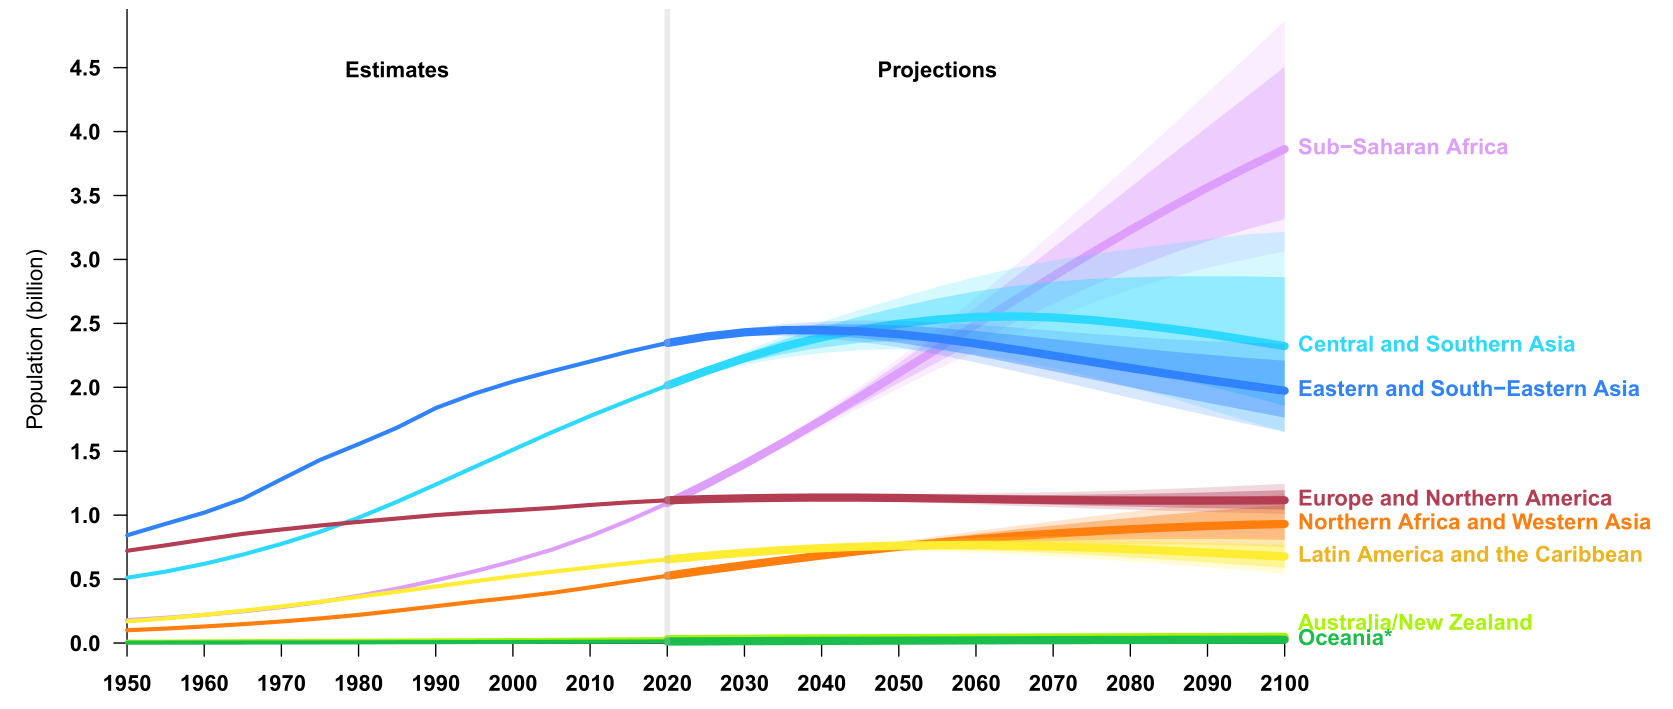
\includegraphics[width=1.0\textwidth]{example_of_logistic.png}
	\caption{Population projection by United Nation using Logistic model}\label{fig:logst_eg}
\end{figure}
\subsection{Autoregression Based on Difference Sequence}
The problem is that the Logistic model has three parameters, and the usual non-linear regression technique mainly solves the model fitting problem of two parameters.Therefore, scientific estimation of the parameters of the Logistic model is a key step for its effective application. Therefore we apply Binary Nonlinear Autoregression Based on Difference Sequence to get the solution of the coefficients.
\\Discretizing Equation (3) we get:
\begin{equation}
	{\frac{{\Delta {y_t}}}{{\Delta t}} = \frac{{{y_t} - {y_{t - 1}}}}{{\Delta t}} = b{y_{t - 1}}(1 - \frac{{{y_{t - 1}}}}{{{y^*}}})}
\end{equation}
This results in two nonlinear autoregressive equations. One is:
\begin{equation}
	{\Delta {y_t} = b\Delta t{y_{t - 1}} - \frac{{b\Delta t}}{{{y^*}}}{y^2}_{t - 1}}
\end{equation}
The other is:
\begin{equation}
	{{y_t} = (1 + b\Delta t){y_{t - 1}} - \frac{{b\Delta t}}{{{y^*}}}{y^2}_{t - 1}}
\end{equation}
Equations (5) and (6) are both non-linear equations, but they are easily converted into linear equation expressions, so that the model parameters are estimated by means of linear regression analysis based on least squares. For linearizable mathematical models, the classic least squares framework can generally be used to determine model parameters.

However, the process of model linearization often causes random perturbations to be transformed, so that the spherical normal distribution of errors is destroyed. Linear regression analysis methods are no longer suitable, and weighted least squares must be used instead. Linear regression will only continue to apply when constant variance occurs after the data set transformation.

However, for equations (5) and (6), the linearization transformation is very simple, and only the quadratic square term ${y_{t-1}^{2}}$ needs to be regarded as a variable. The residual of the model has not undergone any transformation, so the above does not exist. problem. In this case, you can use ${y_{t-1}}$ and ${y_{t-1}^{2}}$ as independent variables, and use ${\Delta y_{t}}$ and ${y_{t}}$ as dependent variables, respectively, to perform a binary linear regression-essentially a nonlinear binary autoregression. With the help of regression analysis, two regression coefficients can be obtained.
\begin{equation}
	{u = b\Delta t\		 or\	 {\rm{u}} = 1 + b\Delta t}
\end{equation}
\begin{equation}
	{v = \frac{{b\Delta t}}{{{y^*}}}}
\end{equation}
Based on this, the model parameter ${b}$ and the saturation value ${y^*}$ are determined, and then the parameter ${a}$ is obtained by using equation (2). The logistic model is fully established.

\begin{figure}[H]
	\centering
	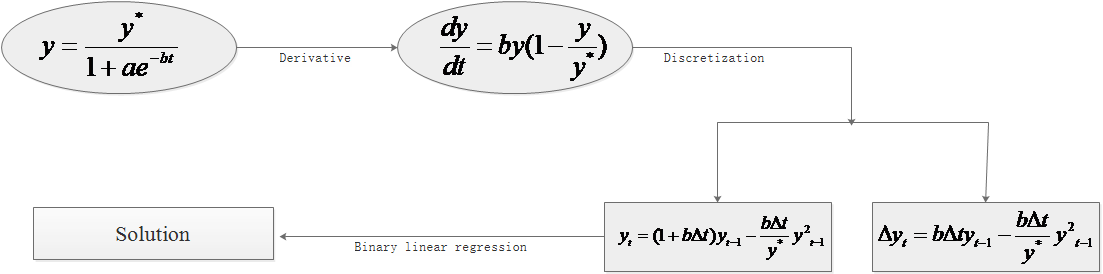
\includegraphics[width=0.9\textwidth]{Logst_rt.png}
	\caption{Mind map presenting the process of finding solutions}\label{fig:Logst_rt}
\end{figure}
\subsection{Solution and Visualization}
We found China's population data from 1999 to 2018. From the scatter plot and preliminary fitting analysis, we know that the changes of data obey the basic characteristics of Logistic growth. Starting from the original data, we can generate 4 columns of data, or 4 variables, ${P_{t-1}}$ is the registered population of the calendar year 1999 to 2017; ${P_{t-1}^{2}}$ is the square of the registered population of the year 1999 to 2017; Pt is the registered population from 2000 to 2018; ${\Delta P_{t}}$ = ${P_{t}-P_{t-1}}$ is the difference between the registered population from 1999 to 2017.
\begin{table}[H]
	\centering
	\caption{China population data and conversion results}
	\begin{tabular}{rrrrr}
		\toprule
		\multicolumn{1}{c}{Year} & \multicolumn{1}{c}{${P_{t-1}}$} & \multicolumn{1}{c}{${P_{t-1}^{2}}$} & \multicolumn{1}{c}{${P_{t}}$} & \multicolumn{1}{c}{${\Delta P_{t}}$} \\
		\midrule
		2000  & 1257860000 & 1582211779600000000  & 1267430000 & 9570000 \\
		2001  & 1267430000 & 1606378804900000000  & 1276270000 & 8840000 \\
		2002  & 1276270000 & 1628865112900000000  & 1284530000 & 8260000 \\
		2003  & 1284530000 & 1650017320900000000  & 1292270000 & 7740000 \\
		2004  & 1292270000 & 1669961752900000000  & 1299880000 & 7610000 \\
		2005  & 1299880000 & 1689688014400000000  & 1307560000 & 7680000 \\
		2006  & 1307560000 & 1709713153600000000  & 1314480000 & 6920000 \\
		2007  & 1314480000 & 1727857670400000000  & 1321290000 & 6810000 \\
		2008  & 1321290000 & 1745807264100000000  & 1328020000 & 6730000 \\
		2009  & 1328020000 & 1763637120400000000  & 1334500000 & 6480000 \\
		2010  & 1334500000 & 1780890250000000000  & 1340910000 & 6410000 \\
		2011  & 1340910000 & 1798039628100000000  & 1347350000 & 6440000 \\
		2012  & 1347350000 & 1815352022500000000  & 1354040000 & 6690000 \\
		2013  & 1354040000 & 1833424321600000000  & 1360720000 & 6680000 \\
		2014  & 1360720000 & 1851558918400000000  & 1367820000 & 7100000 \\
		2015  & 1367820000 & 1870931552400000000  & 1374620000 & 6800000 \\
		2016  & 1374620000 & 1889580144400000000  & 1382710000 & 8090000 \\
		2017  & 1382710000 & 1911886944100000000  & 1390080000 & 7370000 \\
		2018  & 1390080000 & 1932322406400000000  & 1395380000 & 5300000 \\
	\end{tabular}%
	\label{tab:china_data}%
\end{table}%
From the mathematical derivation of Section 1, we know(${\Delta t=1}$):
\begin{equation}
	{\Delta P_{t}=b P_{t-1}-\frac{b}{P^{*}} P_{t-1}^{2}}
\end{equation}

Binary linear regression can be performed using the sequences ${P_{t-1}}$ and ${P_{t-1}^{2}}$ as two independent variables and the differential sequence ${\Delta P_{t}}$ = ${P_{t}-P_{t-1}}$ as the dependent variable. The summary of the regression results is shown in Table 2. When the significance level ${\alpha = 0105}$, the correlation coefficient R value, standard error, DW value, ${F}$ statistic and t statistic test can pass.
\begin{figure}[H]
	\centering
	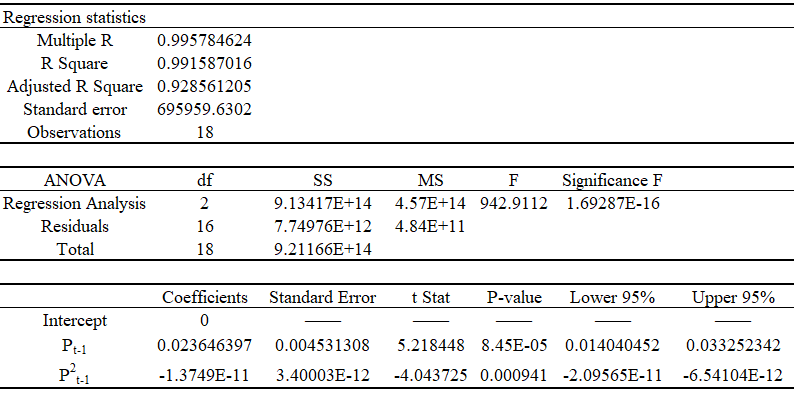
\includegraphics[width=0.9\textwidth]{rst_china.png}
	\caption{Summary output of regression analysis by using difference ${\Delta P_{t}}$ as independent variable}\label{fig:rst_China}
\end{figure}
In the same way we calculate the quantity of native speaker of the top ten languages in 2068 and the data are seen in Appendix 1.

\subsubsection{Conclusion}
We found that the quantity of native speaker of Russian, Portuguese, Spanish and French in the world's top ten predictions for 2018 will decrease in 2068 in comparison of 2018. The current world ’s popular language English and Chinese with the most native speakers still maintained its leading position in 2068, but Chinese growth rate is always higher than English. We think the result fit the big picture that Russia, France, Portugal and spain are now already at or have passed the population peak, facing a population decline. For country like Russia which is in a decline both in economy and world influence meets bigger decline in our model which is consistent with objective facts (From 2018 to 2068, the estimated decline rate is 14.508\% ).The bubble map of 2018 native speaker in comparison with 2068.(Other three maps can be seen in Apendix 3)
\begin{figure}[H]
	\centering
	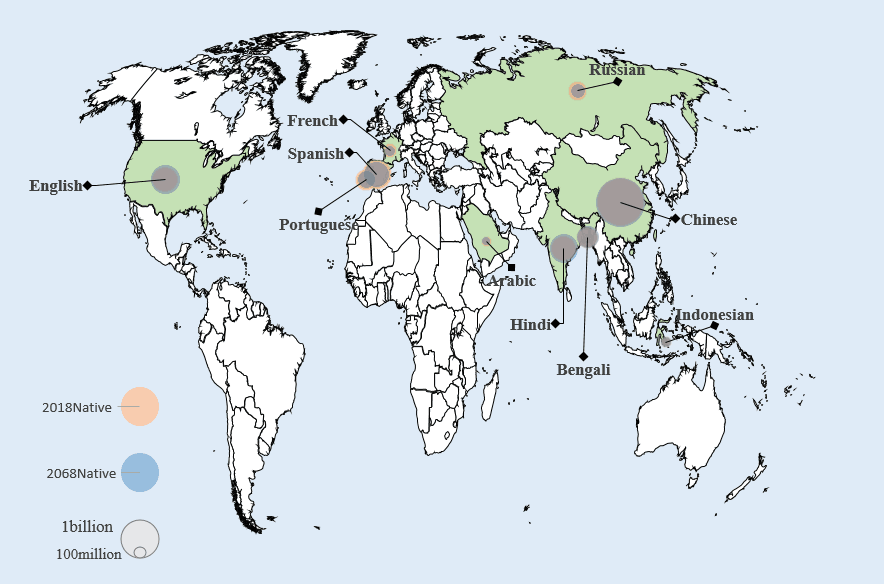
\includegraphics[width=0.9\textwidth]{2018_2068.jpg}
	\caption{Bubble map of Native speakers}\label{fig:2018_2068}
\end{figure}

\subsection{Sensitivity Analysis}
We validate the Logistic model to refrain from changes of coefficients and the turbulence of predicted results for estimated error. The capacity ${y^{*}}$ is stable is the long run so we won’t discuss it.

From euqation (8) we know:
\begin{equation}
{b = \frac{{vy^{*}}}{{{\Delta t}}}}
\end{equation}

${\Delta t}$ is equal to 1, ${y^{*})}$ is a certain value for the same language, so b and ${v}$ are linearly related. The analysis result of ${v}$ under linear regression is very good, so we think that the change in the value of b has little disturbance to the population prediction, so it won't be discussed here.
\subsubsection{Coefficient a}
The maximum possible relative growth rate a is the quotient of y* and the original population ${y_{0}}$ The initial population y0 is randomly chosen, which may induce error . So, we test the sensitivity by valuation. We tested the Mandarin Chinese, for example, in steps of 0.05 from 0.25 to 0.050, and estimated a is 0.36731. The graph is shown below.
\begin{figure}[H]
	\centering
	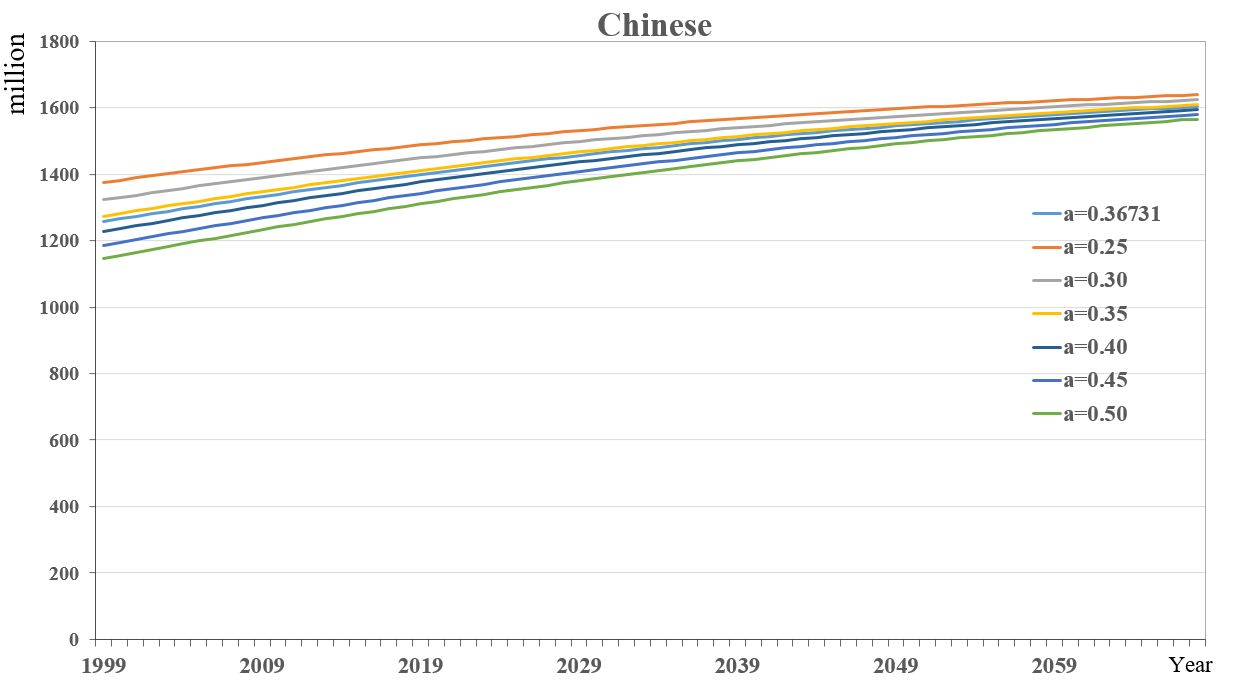
\includegraphics[width=1\textwidth]{sens_china.png}
	\caption{Sensitivity analysis graph of coefficient a}\label{fig:sens_china}
\end{figure}
% Table generated by Excel2LaTeX from sheet 'Sheet1'

The graph in appendix shows that the coefficient a is greatly stable. Given the range, the harmonious situation of native speakers is the same as before for its insulation of the variety of a. And the 50-year prediction bias is below 2.36\%. 
From the results we can know that our model is strongly robust.
\section{Model 2:Geographic distribution}
\subsection{Markov Chain Model}
A Markov chain is "a stochastic model describing a sequence of possible events in which the probability of each event depends only on the state attained in the previous event. 

Markov chain can be described as a random time series,${\left\{ {{\xi _n},n \in T} \right\}}$,where  ${T}$ is a finite set ${\left\{ {1,2....N}\right\}}$,state space ${I = \left\{ {1,2....M} \right\}}$ (${N}$ is the number of discrete time periods, ${M}$ is the number of the discrete state of the event). For any positive integer step ${m}$, and time${\left\{ {1,2....n} \right\} \in T}$ , there is a relation between the corresponding event state i,

We can find that the proportion of the number of people in the second language can be described by the state transition matrix of the Markov chain, so that the number of people using the second language after many years can estimate the transfer trend of each language. Suppose the number of users of the jth second language in year t is ${{y_j}\left( t \right)}$,j = 1,2,3. The probability of switching from the i-th second language to using the j-th second language is${{p_{ij}}}$ , i, j = 1,2,3. The total number of countries is n, and the number of samples we use is t, which is 14-16 years. 4-year data
So the state transition probability matrix is:
\[P = \left[ {\begin{array}{*{20}{c}}
	{{p_{11}}}&{...}&{{p_{1j}}}\\
	{...}&{...}&{...}\\
	{{p_{i1}}}&{...}&{{p_{ij}}}
	\end{array}} \right]\]

The Markov chain prediction model is \[{Y_2} = {Y_1}*P\]

${{Y_1} = {\left[ {\begin{array}{*{20}{c}}
			{{Y_1}(0)}&{...}&{{Y_n}(0)}\\
			{...}&{...}&{...}\\
			{{Y_1}(t - 1)}&{...}&{{Y_n}(t - 1)}
			\end{array}} \right]_{t \times n}}
	{Y_2} = {\left[ {\begin{array}{*{20}{c}}
			{{Y_1}(1)}&{...}&{{Y_n}(1)}\\
			{...}&{...}&{...}\\
			{{Y_1}(t)}&{...}&{{Y_n}(t)}
			\end{array}} \right]_{t \times n}}}$

Available by least squares,
\[P = {(Y_1^T{Y_1})^{ - 1}}Y_1^T{Y_2}\] 
\subsection{Solutions and simulation image}
Available from the previous model ,result after fifty years is
\[{Y_{50}} = {Y_1}*{P^{50}}\]
By adding the changes of the number of second languages speakers we get the
changes of total languages speakers.(Figure 1)




\begin{figure}[H]
	\centering
	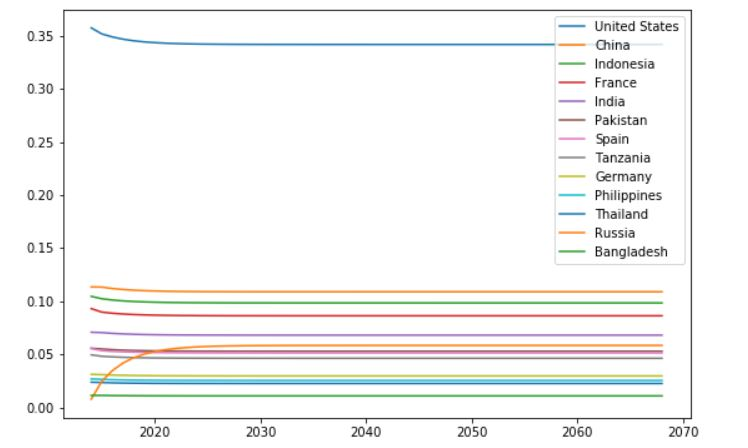
\includegraphics[width=0.9\textwidth]{second_language.jpg}
	\caption{The ratio of simulated second language to its total changed}\label{fig:cnt}
\end{figure}

% Table generated by Excel2LaTeX from sheet 'Sheet1'
\begin{table}[htbp]
	\centering
	\caption{Number of total speakers in 2068 }
	\begin{tabular}{rrrr}
		\toprule
		\multicolumn{1}{l}{English} & \multicolumn{1}{l}{Chinese} & \multicolumn{1}{l}{Indonesia} & \multicolumn{1}{l}{French} \\
		\midrule
		490949418 & 156333833 & 141287077 & 123880799 \\
		\midrule
		\multicolumn{1}{l}{Urdu} & \multicolumn{1}{l}{Spanish} & \multicolumn{1}{l}{Swahili} & \multicolumn{1}{l}{German} \\
		\midrule
		758501056 & 736649541 & 663793234 & 424951760 \\
		\midrule
		\multicolumn{1}{l}{Thai} & \multicolumn{1}{l}{Russian} & \multicolumn{1}{l}{Bengali} &  \\
		\midrule
		322482272 & 837755136 & 154907934 &  \\
		\bottomrule
	\end{tabular}%
	\label{tab:addlabel}%
\end{table}%
Based on the result of the improved Markov model we get the population of the
second language speakers

From the table we can see that, the population of Bengali speakers will increase, and
the rest will decrease.The result shows huge unstability of the prosperity in different
countries, so the languages listed would be replaced by any other languages.

\begin{figure}[H]
	\centering
	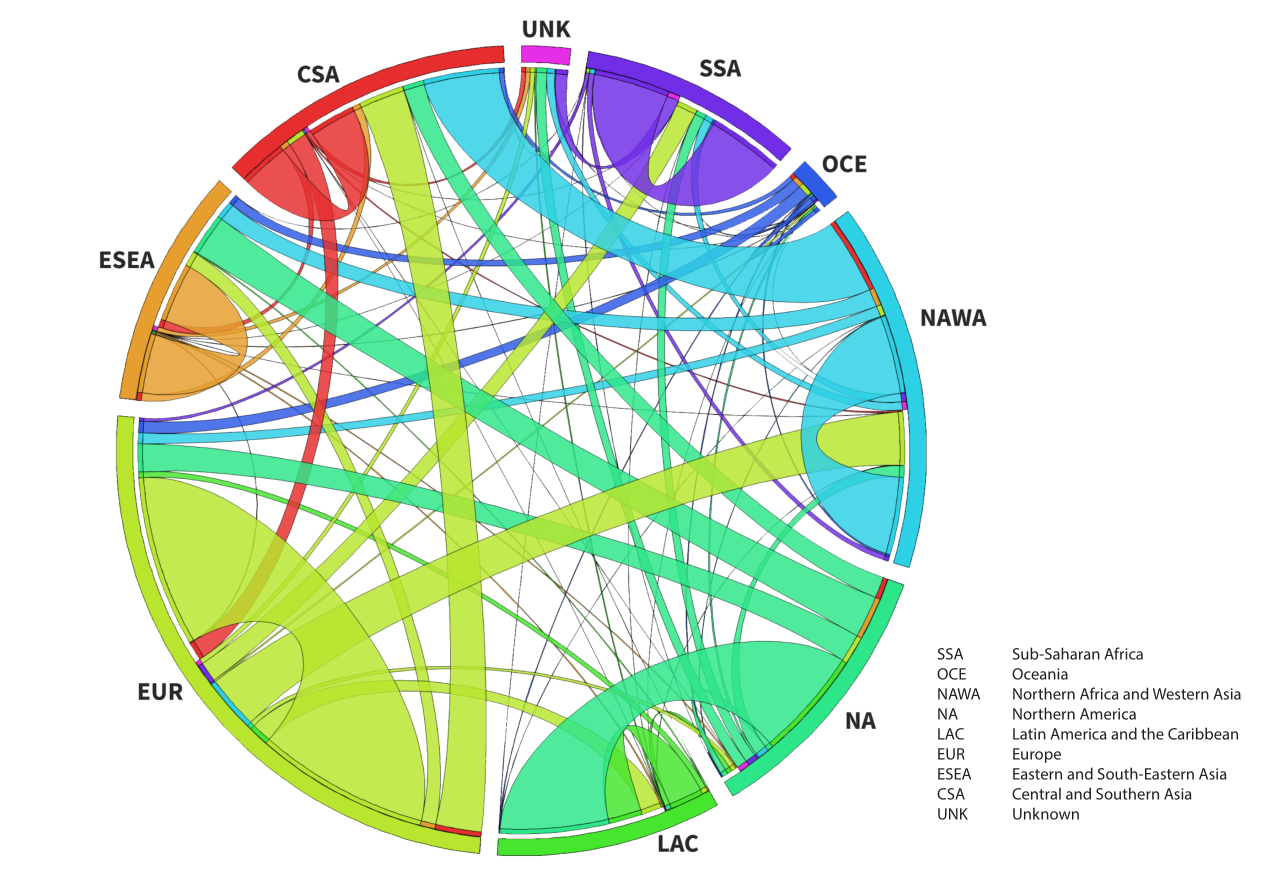
\includegraphics[width=0.8\textwidth]{eye.png}
	\caption{The migration map}\label{fig:eye}
\end{figure}
\subsection{Sensitivity analysis of Markov chain}
Markov chain fine stationary conditions:

First, for a Markov chain to converge, the following conditions must be met:

1. The number of possible states is limited.

2. The transition probability between states needs to be fixed.

3. From any state to any state.

4. It cannot be a simple loop, for example, it is all from x to y and then from y to x.

In our model, the transfer between countries is limited, and the language migration is limited, so it meets the restrictions on object migration in the Markov chain, and the migration probability is calculated from statistical data. It is not simple one-to-one, and our Markov chain is convergent, with a wide range of applications. Excluding a few special cases, the model is less affected.

\section{Model 3: Location Model}
To determine the location of the new offices, we build a location model. Since international branch offices are usually set in well developed countries and countries with potential. On the basis of countries' GDP and their potential, we selected 50 countries as candidates. 

\begin{figure}[H]
	\centering
	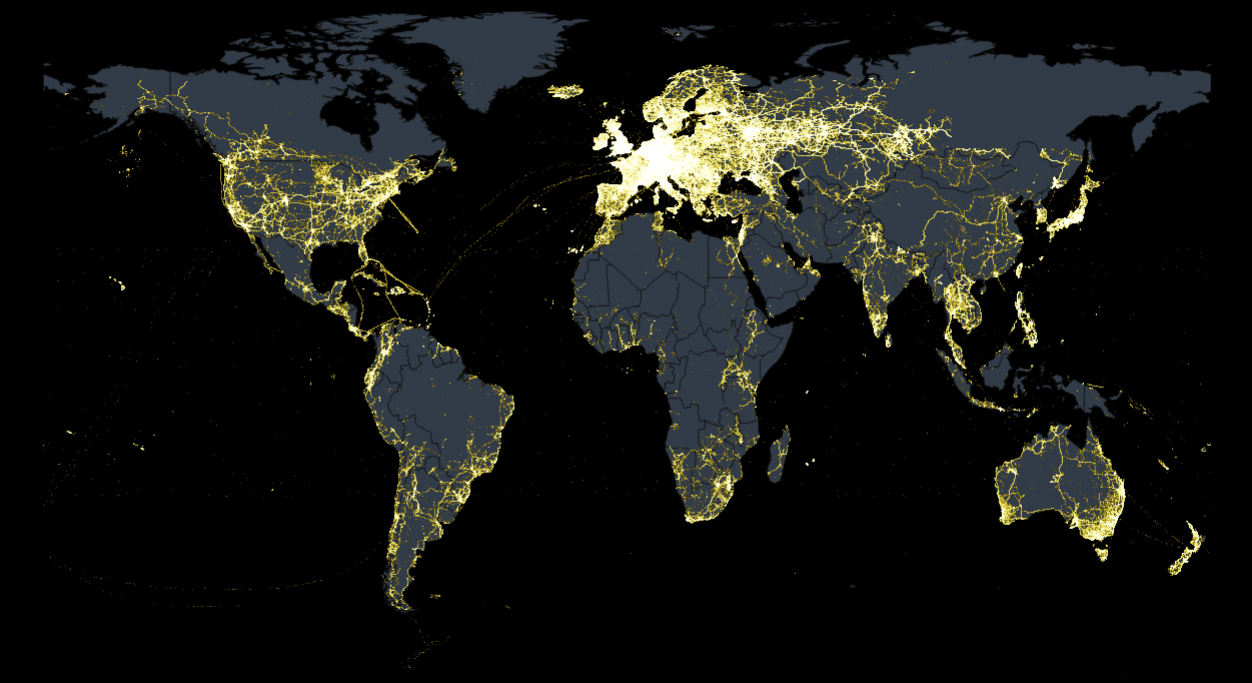
\includegraphics[width=0.9\textwidth]{country_GPS.png}
	\caption{Development in different parts of the world}\label{fig:cnt_GDP}
\end{figure}

This figure reflects the development of each area in the world.

\begin{figure}[H]
	\centering
	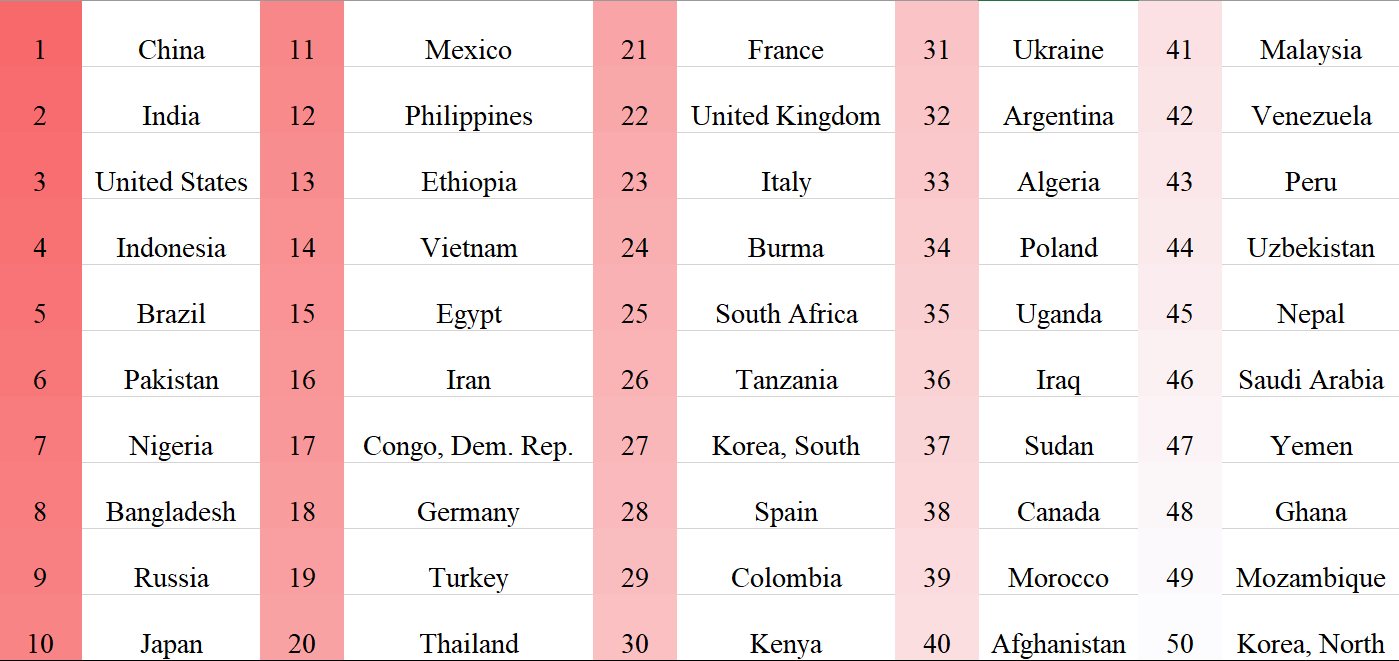
\includegraphics[width=0.9\textwidth]{countries.png}
	\caption{50 candidate countries}\label{fig:cnt}
\end{figure}

Since China and USA had been selected as the office locations, our model is for the remaining 48 countries.

We use the topsis method to determine the office location, and use the entropy method, CRITIC method, and Standard deviation method to set the corresponding weights for each indicator. After the office location is initially determined, we use k-means clustering analysis to determine the office service area. After that, a series of indicators were used to re-score the service effect of different office locations and office areas, and comprehensively determine the best office locations and number. Here are the flow chart of our model:
\begin{figure}[H]
	\centering
	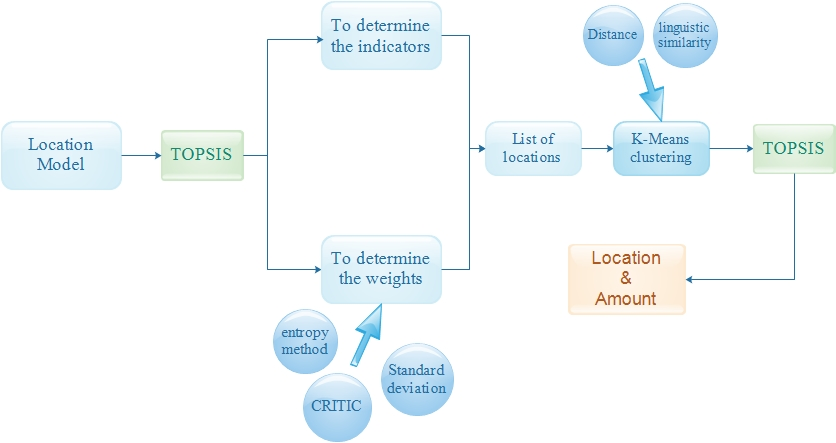
\includegraphics[width=0.8\textwidth]{process.jpg}
	\caption{flow chart of our model}\label{fig:flow_chart}
\end{figure}
\subsection{Weighted-Topsis for location}

In TOPSIS method, "ideal solution" and "negative ideal solution" are the two basic concepts of TOPSIS method. The so-called ideal solution is a conceived optimal solution (scheme), each attribute value of which reaches the best value of each alternative; the negative ideal solution is a conceived worst solution (scheme), it Each attribute value of is the worst value in each alternative. The rule for ordering the schemes is to compare the alternatives with the ideal solution and the negative ideal solution. If one of the schemes is closest to the ideal solution and at the same time is far away from the negative ideal solution, the scheme is the best solution among the alternatives.

In the Weighted-Topsis method in our model, there are 2 types of the indicators:

\begin{table}[H]
	\begin{center}
		\caption{2-types of the indicators in our model}
		\begin{tabular}{|c|c|}
			\hline
			Benefit indicator & The goal is to maximize the indicator  \\ \hline
			Cost indicator    & The goal is to miniimize the indicator \\ \hline
		\end{tabular}
	\end{center}
\end{table}

According to the indicators given in the title and our considerations, we finally chose 6 indicators. They reflect a series of comprehensive factors such as market, cost, language, service range, etc., and can well consider whether an address is suitable as an office. Here are our indicators:

\begin{figure}[H]
	\centering
	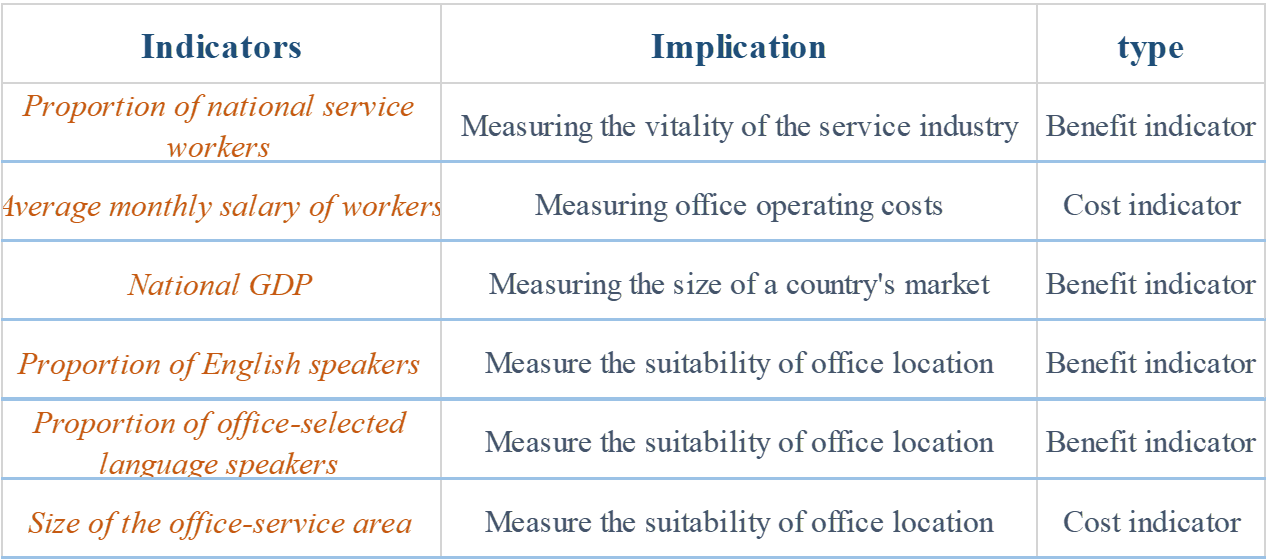
\includegraphics[width=1.0\textwidth]{indicators.png}
	\caption{indicators of our model}\label{fig:indicators}
\end{figure}

The Proportion of national service workers, Average monthly salary of workers, National GDP and Proportion of English speakers are used in our first layer of the topsis, and the Proportion of office-selected language speakers and Size of the office-service area are added in the second layer of the topsis after the area has been clustered by K-means method.

The following paragraphs describe the steps to use topsis on our model.

\begin{enumerate}[\bfseries 1.]
	\item \textbf{Unified indicator type.}
	
	Turn all indicators into benefit indicators. The second indicator and the last indicator of our model are the cost indicator, we need to turn them into benefit indicator by using:
	\begin{equation}
		\max  - x
	\end{equation}
	After this, we can get forward matrix X.
	
	\item \textbf{Standardized forward matrix}
	
	In order to eliminate the influence of different index dimensions, the matrix needs to be processed.
	
	Assume that there are n evaluation objects and m evaluation indexes that have been forwarded. The forward matrix formed is as follows:
	\begin{equation}
		X = \left[ {\begin{array}{*{20}{c}}
				{{x_{11}}}&{{x_{12}}}& \cdots &{{x_{1m}}}\\
				{{x_{21}}}&{{x_{22}}}& \cdots &{{x_{2m}}}\\
				\vdots & \vdots & \ddots & \vdots \\
				{{x_{n1}}}&{{x_{n2}}}& \cdots &{{x_{nm}}}
		\end{array}} \right]\
	\end{equation}
	The matrix to which it is normalized is called Y, and for each element ${y_{ij}}$ in Y:
	\begin{equation}
		{y_{ij}} = \frac{{{x_{ij}}}}{{\sqrt {\sum\limits_{i = 1}^n {{x_{ij}}^2} } }}
	\end{equation}
	
	\item \textbf{Calculate weighted matrix}
	
	Because the impact of each indicator is different, we need to assign a value to each indicator. The weighted matrix is called Z, and each element in Z:
	\begin{equation}
		{z_{ij}} = {w_i} \times {y_{ij}}
	\end{equation}
	We will discuss the method of empowerment later.
	
	\item \textbf{Calculate score and normalize}
	
	After the above steps, we get the weighted normalized matrix Z:
	\begin{equation}
		Z = \left[ {\begin{array}{*{20}{c}}
				{{z_{11}}}&{{z_{12}}}& \cdots &{{z_{1m}}}\\
				{{z_{21}}}&{{z_{22}}}& \cdots &{{z_{2m}}}\\
				\vdots & \vdots & \ddots & \vdots \\
				{{z_{n1}}}&{{z_{n2}}}& \cdots &{{z_{nm}}}
		\end{array}} \right]
	\end{equation}
	
	Define maximum value ${Z^ + }$ and minimum value ${Z^ -}$:
	\begin{equation}
		\begin{array}{l}
			{Z^ + } = \left( {{Z_1}^ + ,{Z_2}^ + , \cdots {Z_m}^ + } \right)\\
			= \left( {\max \left\{ {{z_{11}},{z_{21}}, \cdots ,{z_{n1}}} \right\},\max \left\{ {{z_{12}},{z_{22}}, \cdots ,{z_{n2}}} \right\}, \cdots ,\max \left\{ {{z_{1m}},{z_{2m}}, \cdots ,{z_{nm}}} \right\}} \right)\\
			\\
			{Z^ - } = \left( {{Z_1}^ - ,{Z_2}^ - , \cdots {Z_m}^ - } \right)\\
			= \left( {\min \left\{ {{z_{11}},{z_{21}}, \cdots ,{z_{n1}}} \right\},\min \left\{ {{z_{12}},{z_{22}}, \cdots ,{z_{n2}}} \right\}, \cdots ,\min \left\{ {{z_{1m}},{z_{2m}}, \cdots ,{z_{nm}}} \right\}} \right)
		\end{array}
	\end{equation}
	
	Define the distance between the i-th $\left( {i = 1,2, \cdots ,n} \right)$ evaluation object and the maximum value as ${D_i}^ + $:
	\begin{equation}
		{D_i}^ +  = \sqrt {\sum\limits_{j = 1}^m {{{\left( {{Z_j}^ +  - {z_{ij}}} \right)}^2}} }
	\end{equation}
	
	Define the distance between the i-th $\left( {i = 1,2, \cdots ,n} \right)$ evaluation object and the minimum value as ${D_i}^ - $:
	\begin{equation}
		{D_i}^ -  = \sqrt {\sum\limits_{j = 1}^m {{{\left( {{Z_j}^ -  - {z_{ij}}} \right)}^2}} }
	\end{equation}
	
	Then we can calculate the score of the i-th $\left( {i = 1,2, \cdots ,n} \right)$ evaluation object ${S_i}$:
	\begin{equation}
		{S_i} = \frac{{{D_i}^ - }}{{{D_i}^ -  + {D_i}^ + }}
	\end{equation}
\end{enumerate}

Next we explain how to weight indicators.

Entropy Method, Standard Deviation, CRITIC---The principle of these three methods is based on the degree of variation of the indicator. When the degree of variation of the indicator is smaller, the amount of information reflected is less and the corresponding weight is lower. 

Since the weights given in one way may have large deviations, we combine the three methods to give weights, and analyze the deviations to give the index weights in two ways, which give less deviation.

\begin{itemize}
	\item \textbf{Entropy Method}
	
	Let m indicators of n evaluation objects have been normalized as $y_{ij} \left( {i = 1,2, \cdots ,n;j = 1,2, \cdots m} \right)$. The information entropy of the j-th index is:
	\begin{equation}
		{E_j} =  - \frac{{\sum\limits_{i = 1}^n {{p_{ij}}\ln {p_{ij}}} }}{{\ln n}}\left( {i = 1,2, \cdots ,n;j = 1,2, \cdots ,m} \right)
	\end{equation}
	and ${p_{ij}} = \frac{{{y_{ij}}}}{{\sum\limits_{i = 1}^n {{y_{ij}}} }}$.
	When E is smaller, the difference between the data is larger, so the larger the information provided, the greater the weight of the indicator, and vice versa.
	
	Then we can get the calculation formula of objective weight:
	\begin{equation}
		{w_j} = \frac{{1 - {E_j}}}{{m - \sum\limits_{j = 1}^m {{E_j}} }}(j = 1,2, \cdots m)
	\end{equation}
	
	\item \textbf{Standard Deviation}
	
	Unlike the calculation of information entropy, in the standard deviation method, we use the method of calculating standard deviation to measure the amount of information provided by an indicator. When the standard deviation is large, we think that it provides more information. When the standard deviation is small, we think it provides less information.
	
	The calculation as following:
	\begin{equation}
		{w_j} = \frac{{{\sigma _j}}}{{\sum\limits_{j = 1}^m {{\sigma _j}} }}(j = 1,2, \cdots ,m)
	\end{equation}
	where $\sigma _j$ represents the standard deviation.
	
	\item \textbf{CRITIC}
	
	The CRITIC method weights indicators based on two basic concepts: The first is contrast. When the standard deviation is larger, the weight is relatively larger. The second is to evaluate the conflict between indicators. Here we introduce the correlation coefficient r between indicators. When there is a strong positive correlation between indicators, it means that the conflict between the two indicators is low, and the information reflected by the two indicators is relatively similar. When there is a strong negative correlation between the two indicators, it means that the conflict between the two indicators is large, and the information reflected by the two indicators is quite different.
	
	The calculation as following:
	
	The amount of information contained in the j-th indicator is:
	\begin{equation}
		{c_j} = {\sigma _j}\sum\limits_{i = 1}^m {(1 - {r_{ij}})(j = 1,2, \cdots ,m)} 
	\end{equation}
	where ${r_{ij}}$ represents the correlation coefficient between the i-th indicator and j-th indicator.
	
	Then we get the j-th indicator's weight:
	\begin{equation}
		{w_j} = \frac{{{c_j}}}{{\sum\limits_{i = 1}^m {{c_i}} }}(j = 1,2, \cdots ,m)
	\end{equation}
\end{itemize}

\subsection{Weighted K-Means Clustering for area}
After the first usage of the Weighted-Topsis, we get the score of each country among the 50-countries' list. Considering that each office needs to serve an area, we introduce Weighted K-Means Clustering to determine the area that one office needs to serve.

K-means is a certain distance from the data point to the prototype as the objective function of the optimization, and the method of calculating the extreme value of the function is used to obtain the adjustment rule of the iterative operation. The K-means algorithm uses Euclidean distance as a similarity measure. It seeks the optimal classification corresponding to a certain initial clustering center vector MC, so that the evaluation index D is minimized. The algorithm uses the sum of squared error function as the clustering criterion function. Eventually, the obtained clusters satisfy the similarity of objects in the same cluster, and the cluster center and the objects assigned to them represent a cluster.

\begin{figure}[H]
	\centering
	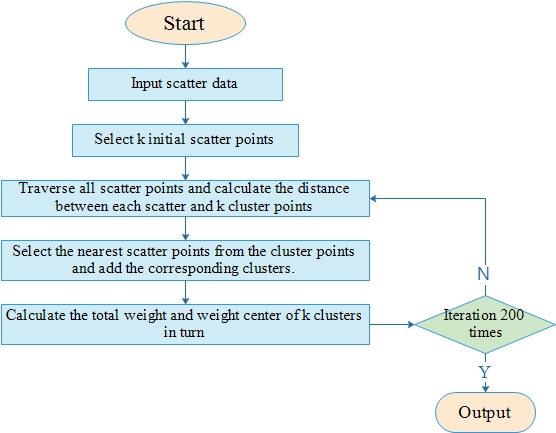
\includegraphics[width=0.7\textwidth]{K-means.jpg}
	\caption{flow chart of K-Means Clustering}\label{fig:K-means}
\end{figure}

The core formula of the K-means algorithm:
\begin{equation}
	D\left( {\left\{ {{\pi _c}} \right\}_{c = 1}^k} \right) = \sum\limits_{c = 1}^k {\sum\limits_{a,e{x_c}} {{{\left\| {{a_i} - {m_c}} \right\|}^2}} } ,{\rm{ where }}{m_c} = \frac{{\sum\limits_{a, \in {\pi _c}} {{a_i}} }}{{\left| {{\pi _c}} \right|}}
\end{equation}
${a_{ij}},\left( {i = 1,2,...,n;j = 1,2,...,m} \right)$ refers to all of the elements. And here m=2, means the longitude and latitude, which is the location of the center point(At first is the office selected.). ${\pi _c}$ means the cluster group and the total number is k. ${m_c}$ is the cluster center of the element ${a_i}$ in group ${\pi _c}$. After continuous iteration we can get the final clustering result.

Through the k-means algorithm, we can obtain a good regionalization scheme from the initial center point and continuous iteration. Here is an example:

\begin{figure}[H]
	\begin{minipage}[t]{0.3\linewidth}
		\centering
		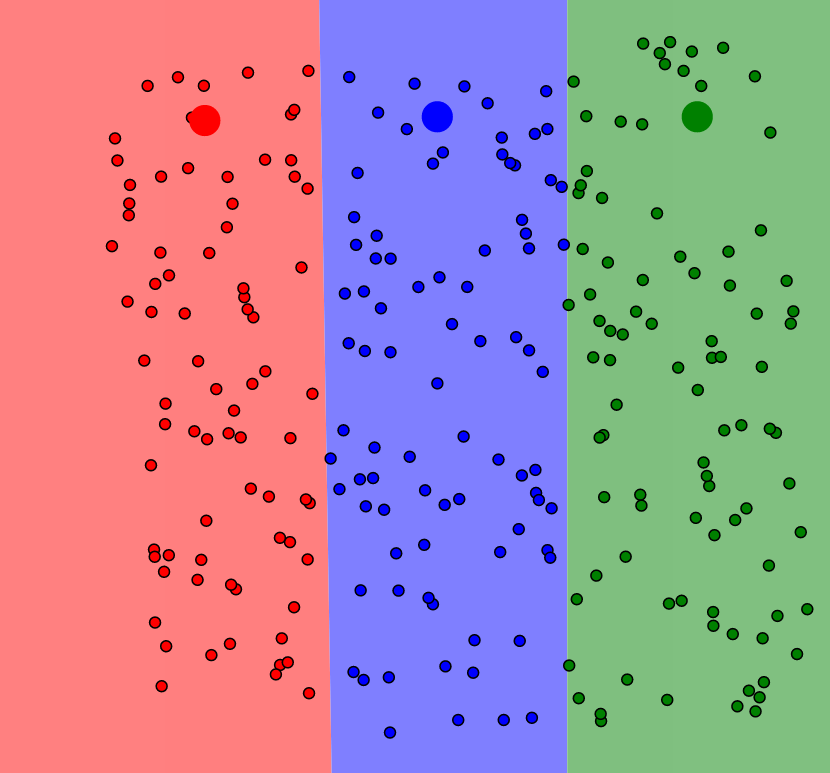
\includegraphics[height=4cm,width=4cm]{k-means_1.png}
		\caption{Init}
	\end{minipage}%
	\hfill
	\begin{minipage}[t]{0.3\linewidth}
		\centering
		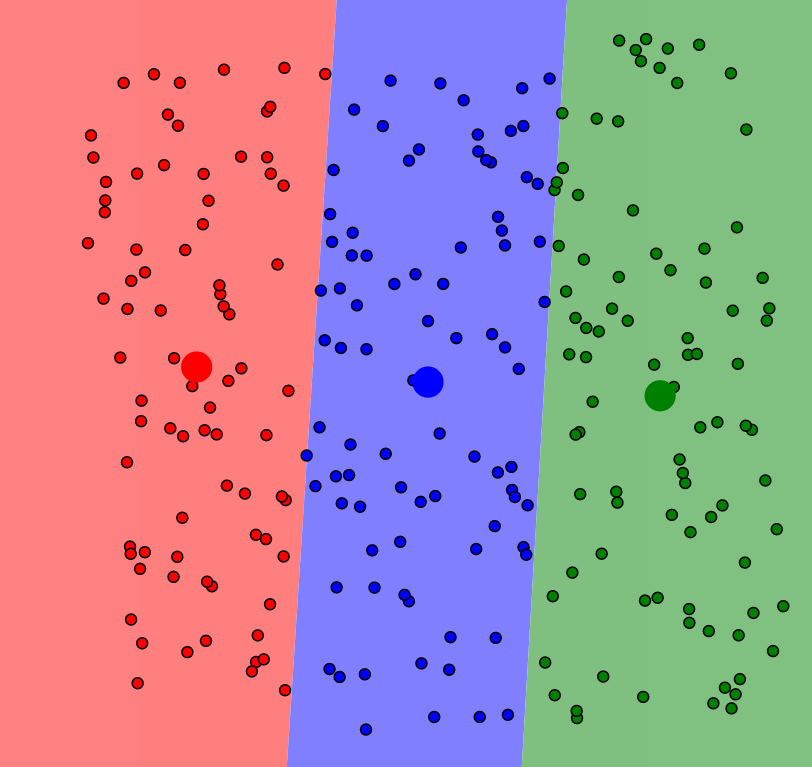
\includegraphics[height=4cm,width=4cm]{k-means_2.png}
		\caption{After 10 iterations}
	\end{minipage}
	\hfill
	\begin{minipage}[t]{0.3\linewidth}
		\centering
		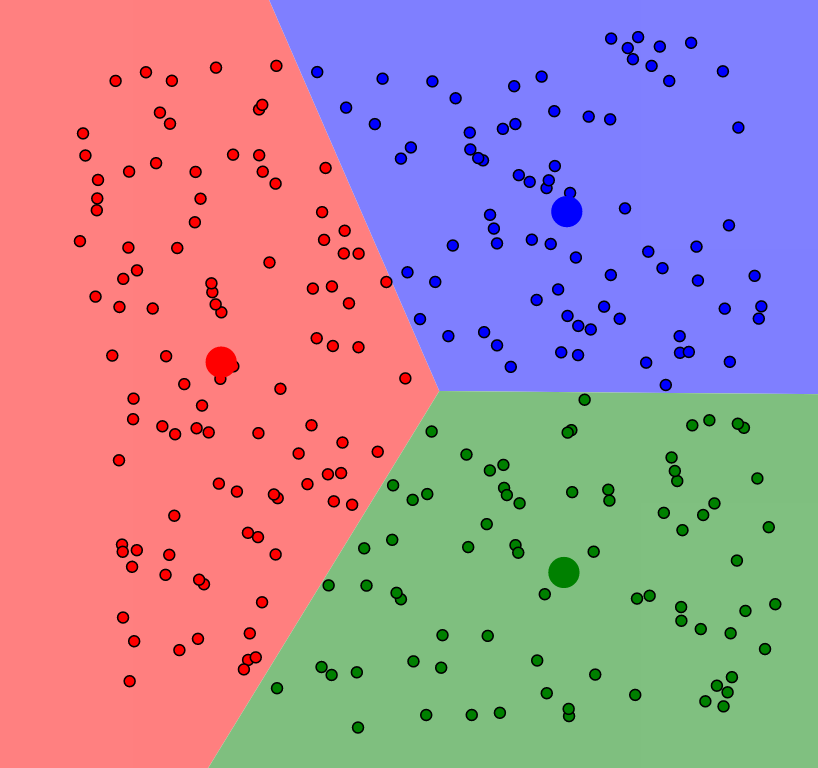
\includegraphics[height=4cm,width=4cm]{k-means_3.png}
		\caption{After 50 iterations}
	\end{minipage}
\end{figure}

From the example we can see the cluster center in the final cluster compared to the original has a large offset. This means the K-Means clustering is not enough to solve our location model. Since the K-means clustering model uses a 1: 1 ratio for the distance comparison of each scattered point set, but for us, we need to consider not only the straight line distance between the capital and the cluster center, but also to the language similarity and other factors. If we use distance as the sole criterion, then it is better to define the service area according to the radiation range centered on the country. Because then the office location we originally selected will not change. However, Based on our considerations, the reason we apply the k-means algorithm is as follows:
\begin{itemize}
	\item Introduce language similarity as weights to help us flexibly divide regions.
	\item Judging the correctness and appropriateness of the initial choice by observing the change in the center point. If the center point has a large deviation, it means that the initially selected point is not suitable as an office. Then we can consider changing the location or country for better results.
\end{itemize}

Based on the above ideas, we apply the Weighted K-Means Clustering to solve our model.

The core formula of the Weighted K-means Clustering:
\begin{equation}
	D\left( {\left\{ {{\pi _c}} \right\}_{c = 1}^k} \right) = \sum\limits_{c = 1}^k {\sum\limits_{{a_i} \in {\pi _c}} {w_i^y} } {\left\| {{a_i} - {m_c}} \right\|^2},\quad {\rm{ where }}{m_c} = \frac{{\sum\limits_{a,e{\pi _c}} {w_i^y} {a_i}}}{{\sum\limits_{{a_i} \in {\pi _c}} {w_i^y} }}
\end{equation}
The calculation method of this formula is very similar to the k-means algorithm, except that for different sample points, a corresponding weight wi and a weight attenuation coefficient y are multiplied. Here we set the y=1.


\subsection{Solution and Analysis of Location Model}

Via the data we collected, we quantified six indicators and normalized these indicators. Running the Entropy Method, Standard Deviation, CRITIC respectively. We get three different weight vectors as following:

\begin{center}
	Entropy Method:
	${\left[ {\begin{array}{*{20}{c}}
			{\begin{array}{*{20}{c}}
				{\begin{array}{*{20}{c}}
					{0.22}\\
					{0.25}
					\end{array}}\\
				{0.31}
				\end{array}}\\
			{0.22}
			\end{array}} \right]^{ - 1}}$
	
	Standard Deviation:
	${\left[ {\begin{array}{*{20}{c}}
			{\begin{array}{*{20}{c}}
				{\begin{array}{*{20}{c}}
					{0.14}\\
					{0.39}
					\end{array}}\\
				{0.32}
				\end{array}}\\
			{0.15}
			\end{array}} \right]^{ - 1}}$
	
	CRITIC:
	${\left[ {\begin{array}{*{20}{c}}
			{\begin{array}{*{20}{c}}
				{\begin{array}{*{20}{c}}
					{0.30}\\
					{0.15}
					\end{array}}\\
				{0.35}
				\end{array}}\\
			{0.20}
			\end{array}} \right]^{ - 1}}$
\end{center}

We calculated the rankings obtained by topsis under the three kinds of weights, and finally selected 12 countries. Considering that a country's capital often best reflects its economic level. At the beginning, we assumed that the national capital was the office location. As for the choice of language: we assume the most spoken language in the region other than English as the language the office selected to use.

\begin{figure}[H]
	\centering
	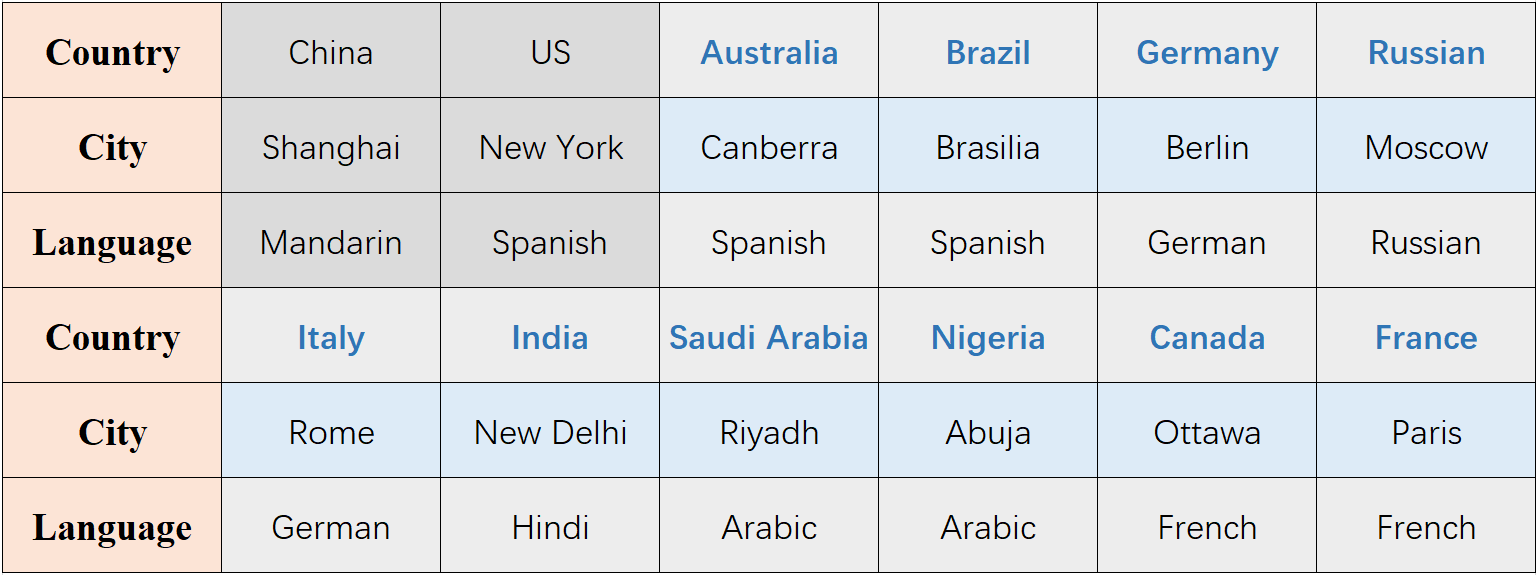
\includegraphics[width=1\textwidth]{first_select.png}
	\caption{Selected location by topsis}\label{fig:first_select}
\end{figure}
Because China and the United States have been selected as office locations, we just need to consider the other 10 regions. The selection of China and the United States also proved the correctness of the first site selection in our model.

After the Weighted-Topsis, we tried the choices of 6 different countries among lists and brought them into the k-means cluster with distance and language consistency and country relations as weights to divide the service area for the selected office. 

Later, the regional division was completed, we brought the next two indicators to recalculate the score of topsis, and selected the highest 6 locations in different divisions by clustering. 

After multiple assignments we found that when we use Germany, Brazil, Australia, Nigeria, Russian and India as the locations of the office, we can receive the highest benifit and lowest cost. The deviation of the cluster center is also little, which means the capital is suitable for the location. And we find that when we use different combination, the 6 highest average scores are also these countries. Here is the score in average:
\begin{figure}[H]
	\centering
	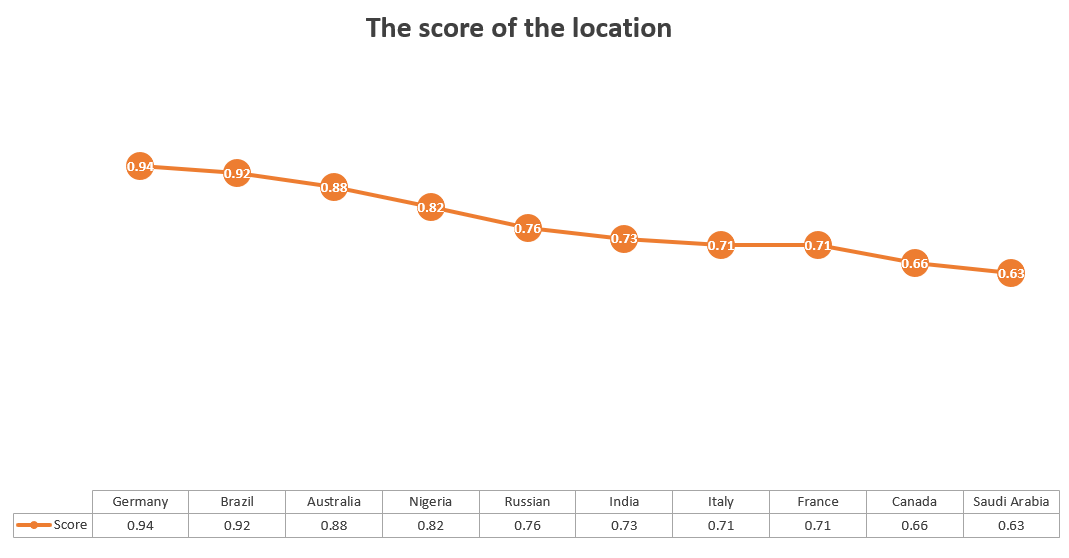
\includegraphics[width=0.9\textwidth]{Location_Score.png}
	\caption{Score of the location}\label{fig:location}
\end{figure}

For determing the best amount of the offices, we just need to make minor changes to our model, since the amount does not affect the score. We can know from the supervisor's analysis that when we cut down the amount of the offices, the office construction costs and operating costs will decrease, but revenue and service intensity will increase. Our indicators take these points into account, so we can continue to use our model rather than change the indicators. Finally, by running our models, we find that building 6 offices in these countries is still the most suitable. At this point, our model is solved, and we give the distribution of our offices in World Map:
\begin{figure}[H]
	\centering
	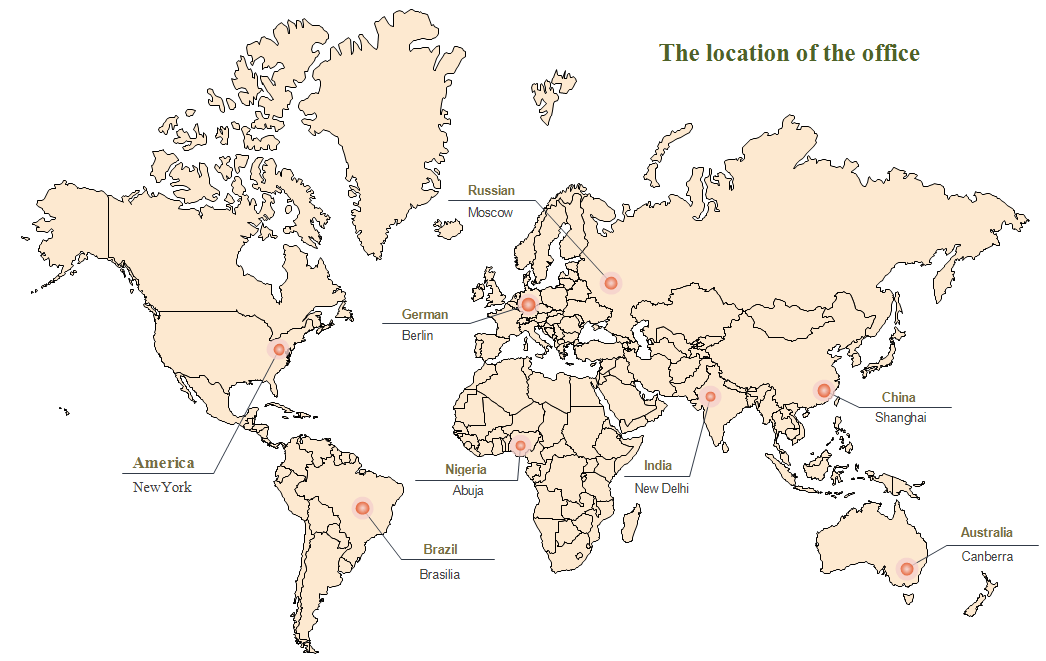
\includegraphics[width=1\textwidth]{location.png}
	\caption{location of the offices}\label{fig:offices}
\end{figure}

\subsection{Sensitivity Analysis}
For problem 2, because our model considers more comprehensive factors, it can be consistent in the short and long term. Here we give a sensitivity analysis on time.

Based on our initial scores, the values and scores of the six selected countries are shown below.

\begin{figure}[H]
	\centering
	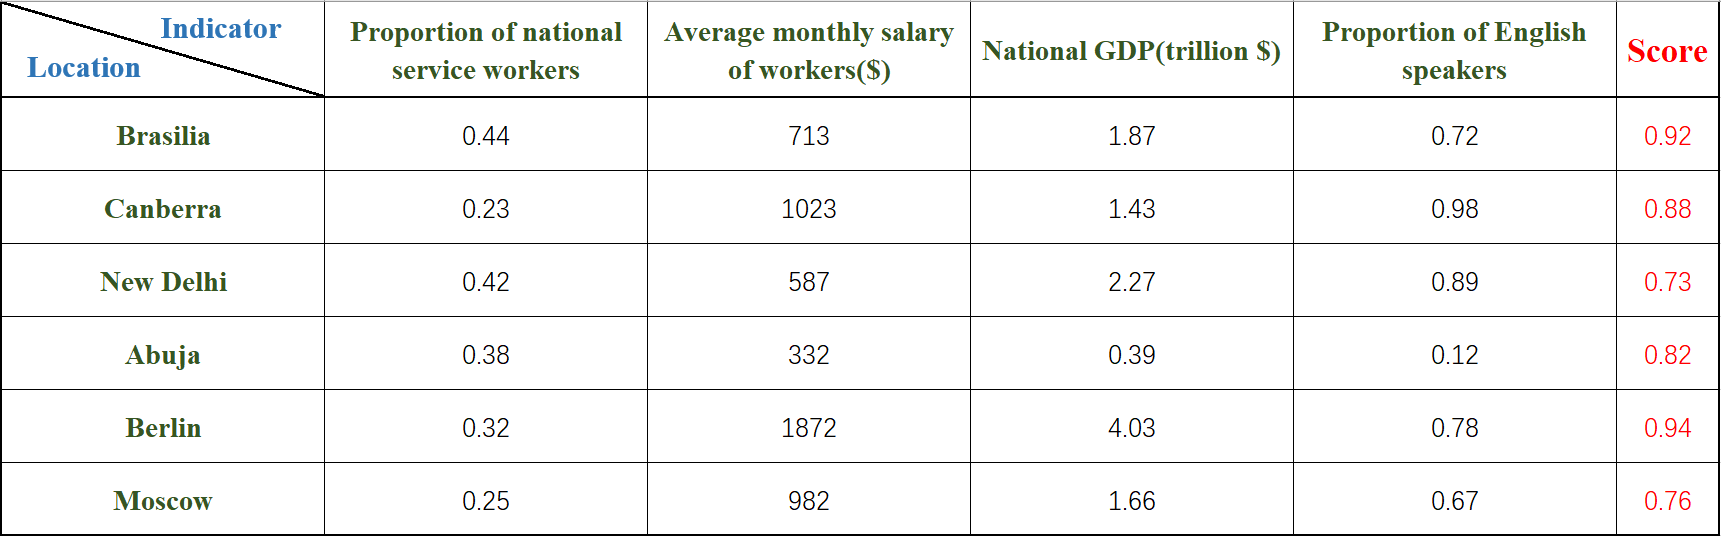
\includegraphics[width=1\textwidth]{Sensitivity.png}
	\caption{Short-term Score}\label{fig:sensitivity}
\end{figure}

According to our analysis, over time, when a country begins to develop, its number of English speakers will increase, and GDP will increase. These are all contributing factors, but the decline in service practitioners and the increase in per capita wages will be restrained. Effect, according to our prediction, this promotion and inhibition effect will maintain the stability of the score. This effect is predictable, because in the initial country selection, we not only considered the current development level of this country, but also considered the potential development potential of developing countries.

\begin{figure}[H]
	\centering
	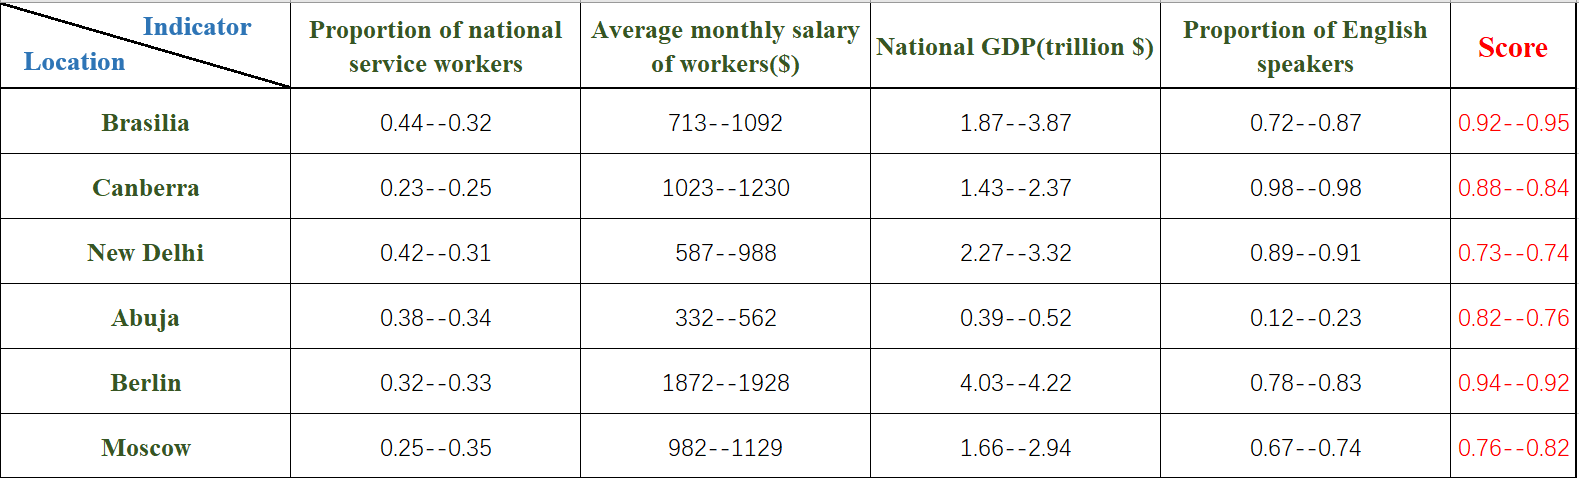
\includegraphics[width=1\textwidth]{Sensitivity_1.png}
	\caption{Long-term Score}\label{fig:sensitivity_1}
\end{figure}

As can be seen from the above figure, in the long-term development process, our best choice is still these six countries, and the scores have not changed much.

\begin{letter}{Memo}
	\begin{flushleft}  % 左对齐环境,无首行缩进
		\textbf{To:} Chief Operating Officer of the service company\\
		\textbf{From:} Team 2006872\\
		\textbf{Date:} February 16th, 2020\\
		\textbf{Subject:} Results and Recommendations on language distribution and offices decision
		\rule{\textwidth}{0.15mm} 
	\end{flushleft}
	We are glad to hear that your company is about to expand your business and build six new offices around the world. We are also honored to be involved in your company's office location and language development research modeling. After four days of modeling work and analysis. Here we give our model and analysis and hope to help your company.
	
	In population model we applied logistic model. Substituting data into the model, we found that the native speakers' quantity of Russian, Portuguese, French and spanish users will decrease in 2068 while other languages continue to increase indicating they may be replaced by other powerful languages. The current world ’s popular language English and Chinese with the most native speakers still maintained its leading position in 2068, but in the later period, Chinese became the most spoken language in the world due to the rise of its second language users and its huge population base over English. In terms of geographical distribution, we construct a transfer matrix description through a Markov chain model. we find that language transmission and geographical distribution are generally regional. Of the top ten languages, except English, Spanish, and French, which are used in a wide range of areas, the other languages are spread only in the certain areas.
	
	Based on the model of language distribution, combined with Algorithm for Fuzzy Clustering method and P-Center method, we develop a Location Model to further provide a recommendation for your company to select the location of your new international office and its working language. Our model takes into account market, cost and language factors. Allows your company to obtain greater benefits at a lower cost. These six locations as well as the languages to be used in the new offices are as the following:
	\begin{figure}[H]
		\centering
		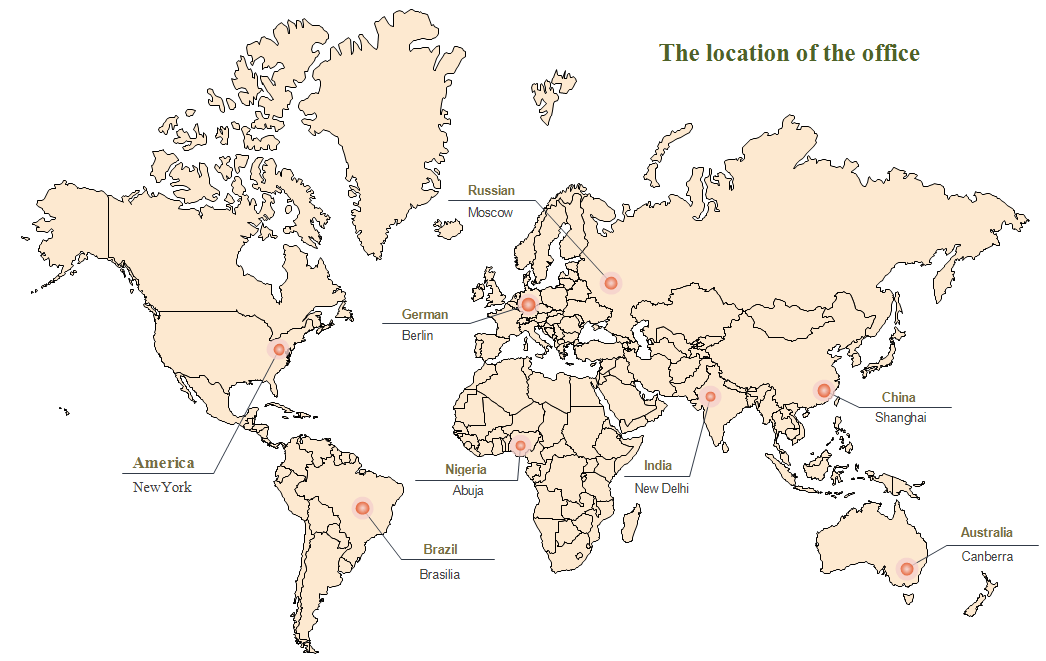
\includegraphics[width=0.9\textwidth]{location.png}
		\caption{Long-term Score}\label{fig:location.png}
	\end{figure}
\begin{figure}[H]
	\centering
	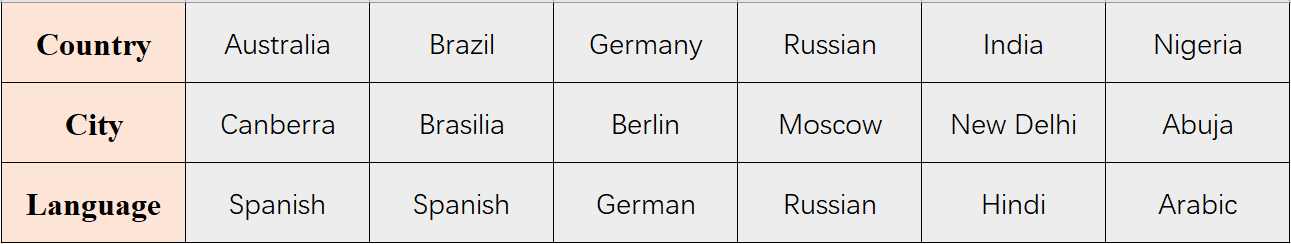
\includegraphics[width=0.9\textwidth]{Distribution.png}
	\caption{Long-term Score}\label{fig:Distribution.png}
\end{figure}
	
	And our model considers the potential factors of the degree of development and has consistency in the short and long term, ensuring that the company can avoid the risk of relocation in the future.
	
	The above is our model, hope our model can help you in your decision.
	
	Best wishes.
	\begin{flushright}
		Yours sincerely,
		
		Team 2006872
	\end{flushright}

\end{letter}
% 参考文献,此处以 MLA 引用格式为例
\begin{thebibliography}{99}
\bibitem{1} \emph{CHEN Yan 2 guang, YU Bin. Three models for predicting population growth. Journal of Central China NormalUni 2versity (Nat. Sci. ) , 2006, 40(3) : 452 - 456.}
\bibitem{2} \emph{Shih H S , Shyur H J , Lee E S . An extension of TOPSIS for group decision making[J]. Mathematical and Computer Modelling, 2007, 45(7-8):801-813.
}
\bibitem{3}\emph{Wong J A H A . Algorithm AS 136: A K-Means Clustering Algorithm[J]. Journal of the Royal Statistical Society. Series C (Applied Statistics), 1979, 28(1):100-108.
}
\bibitem{4}\emph{Daniel Rudolf. Error bounds for computing the expectation by Markov chain Monte Carlo[J].Monte Carlo Methods and Applications, 2010,16(3-4).}
\bibitem{5}\emph{Olson D L. Comparison of weights in TOPSIS models.[M]. 2004.
}
\end{thebibliography}


% 以下为附录内容
% 如您的论文中不需要附录,请自行删除
\begin{subappendices}  % 附录环境

\section{Appendix}
% Table generated by Excel2LaTeX from sheet 'Sheet1'
\begin{table}[htbp]
	\centering
	\caption{Native speaker projection and comparison}
	\begin{tabular}{cccc}
		\toprule
		Country & 2068/million & 2018/million & Difference/million \\
		\midrule
		China & 1604.60  & 1395.38  & 209.22  \\
		US    & 381.25  & 327.17  & 54.09  \\
		UK    & 77.01  & 66.44  & 10.57  \\
		Canada & 58.07  & 37.07  & 21.00  \\
		Australia & 48.81  & 24.90  & 23.91  \\
		Ireland & 5.24  & 4.82  & 0.42  \\
		New Zealand & 5.95  & 4.74  & 1.20  \\
		English/Total & 576.32  & 394.36  & 181.96  \\
		Hindi & 542.80  & 341.20  & 201.60  \\
		Spanish & 420.30  & 460.10  & -39.80  \\
		French & 66.50  & 77.20  & -10.70  \\
		Arabic & 42.30  & 34.30  & 8.00  \\
		Bengali & 327.50  & 228.30  & 99.20  \\
		Russian & 131.40  & 153.70  & -22.30  \\
		Portuguese & 189.30  & 220.70  & -31.40  \\
		Indonesian & 67.30  & 43.30  & 24.00  \\
	\end{tabular}%
	\label{tab:addlabel}%
\end{table}%
\large\textbf{Appendix 2}
\begin{table}[H]
	\centering
	\caption{Sensitivity Analysis about b}
	\begin{tabular}{cccc}
		\toprule
		a     & \multicolumn{1}{p{14.39em}}{ Original value} & \multicolumn{1}{l}{New Projection} & \multicolumn{1}{l}{Bias of Projection} \\
		\midrule
		0.25  & 1604.595977 & 1639.702399 & 2.19\% \\
		0.3   & 1604.595977 & 1624.553786 & 1.24\% \\
		0.35  & 1604.595977 & 1609.682516 & 0.32\% \\
		0.4   & 1604.595977 & 1595.081041 & 0.59\% \\
		0.45  & 1604.595977 & 1580.742086 & 1.49\% \\
		0.5   & 1604.595977 & 1566.658633 & 2.36\% \\
	\end{tabular}%
	\label{tab:sens_b}%
\end{table}%
\end{subappendices}
\large\textbf{Appendix 3}
\begin{figure}[H]
	\centering
	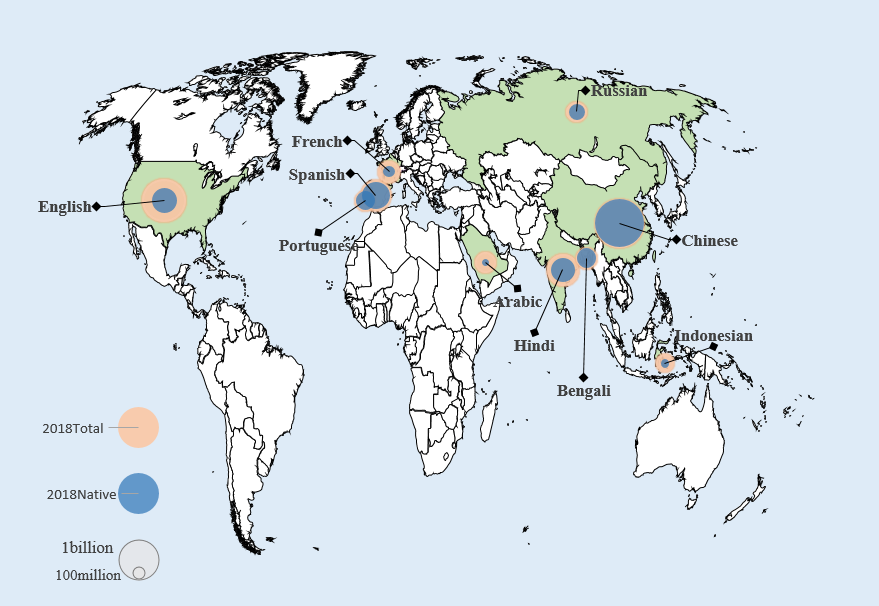
\includegraphics[width=0.8\textwidth]{18t_18n.jpg}
	\caption{2018Total in comparison with 2018Native}\label{fig:18t_18n}
\end{figure}
\begin{figure}[H]
	\centering
	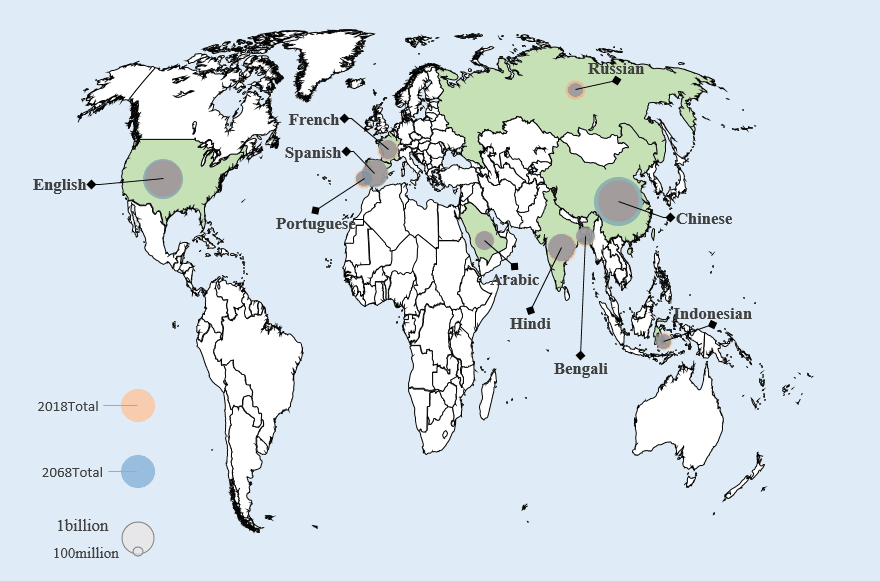
\includegraphics[width=0.8\textwidth]{18t_68t.jpg}
	\caption{2018Total in comparison with 2018Native}\label{fig:18t_68t}
\end{figure}
\begin{figure}[H]
	\centering
	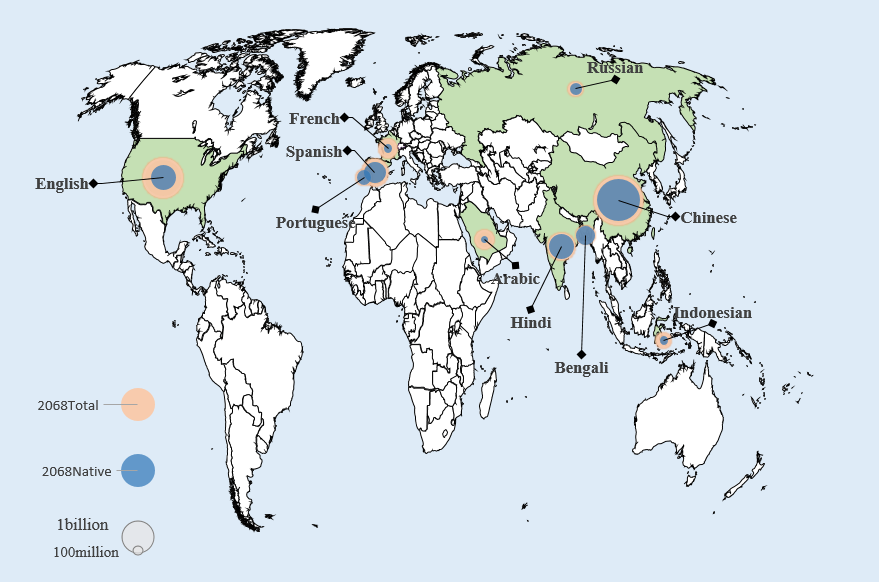
\includegraphics[width=0.8\textwidth]{68t_68n.jpg}
	\caption{2018Total in comparison with 2018Native}\label{fig:68t_68n}
\end{figure}
\large\textbf{Appedix 4}
\begin{figure}[H]
	\centering
	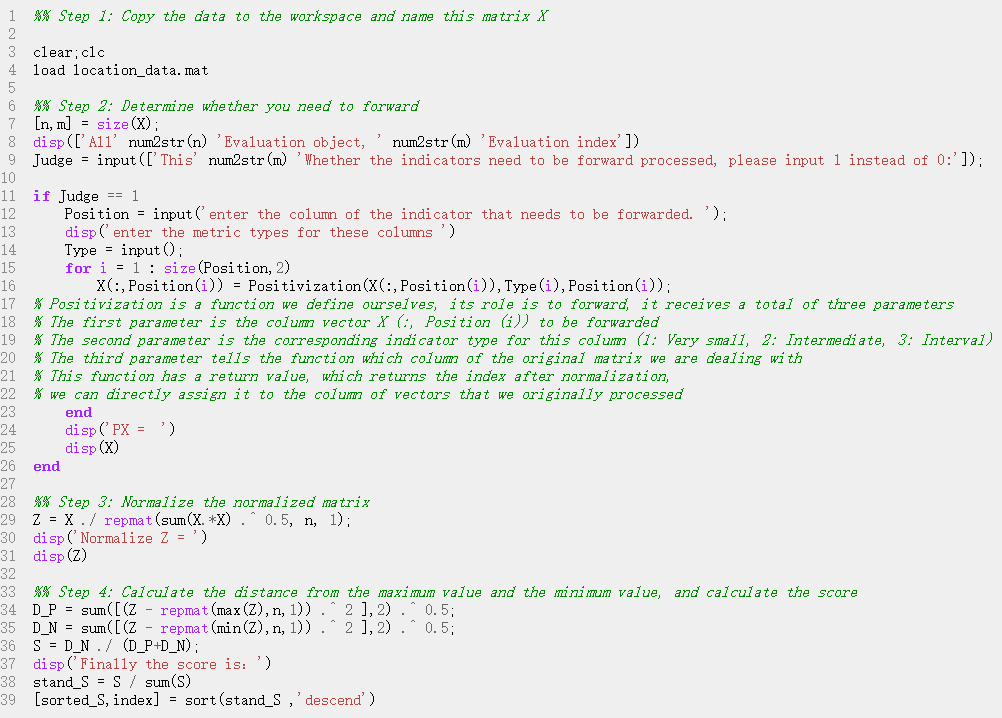
\includegraphics[width=1.0\textwidth]{top.png}
	\caption{Code of TOPSIS}\label{fig:top}
\end{figure}
\end{document}  % 结束